\section{Δίκτυα των Data centers}

Με την αύξηση χρήσης υπηρεσιών cloud, υπηρεσιών πολυμέσων και
γενικών web εφαρμογών τα τελευταία έτη, έχει υπάρξει αντίστοιχη
εκθετική άνοδος στην κίνηση δεδομένων των data ceters. Αυτή η άνοδος
στην κίνηση δημιουργεί προκλήσεις διότι για την εξυπηρέτησή της,
πρέπει να αυξηθεί η χωρητικότητα του δικτύου, χωρίς να αυξηθεί η
καθυστέρηση όπως και, λόγο θερμικών περιορισμών, πρέπει η συνολική
κατανάλωση τις υποδομής του δικτύου να παραμείνει στα ίδια
επίπεδα. Αυτό είναι ολοένα και πιο δύσκολο με την χρήση ηλεκτρονικών
μεταγωγών και γι' αυτόν τον λόγο πληθώρα βιβλιογραφίας υπάρχει για την
χρήση οπτικών μεταγωγέων εντός των data centers \cite{6129370}.

Λόγο της πολύ δύσκολης μεταγωγής πακέτων στο οπτικό πεδίο,
συνδυαστικές λύσεις μπορούν να υλοποιηθούν με οπτική μεταγωγή
κυκλώματος για επικοινωνίες μεταξύ σταθμών και συμβατική μεταγωγή
πακέτων μετά από μετατροπή του οπτικού σήματος σε ηλεκτρικό
\cite{6533163} \cite{Helios}. Τέτοιες υλοποιήσεις
υπάρχουν και έχουν αποδειχθεί πειραματικά πως δεν υστερούν ούτε σε
ταχύτητα ούτε σε απόδοση \cite{6533163}.

\begin{figure}[H]
  \centering
  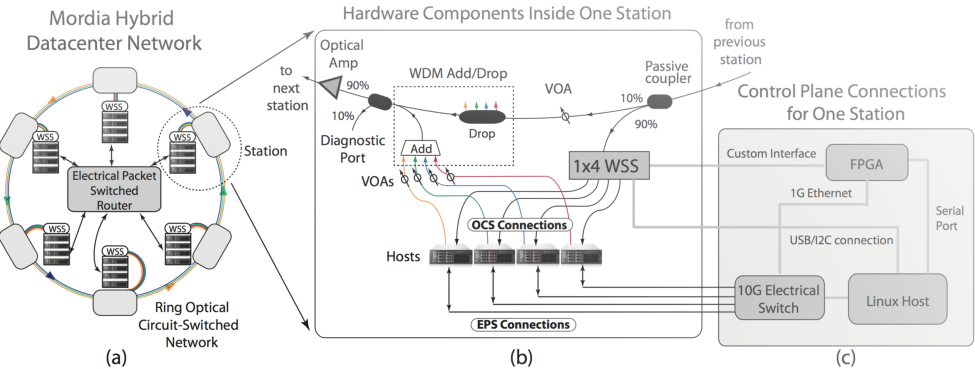
\includegraphics[width=\linewidth]{mordia.pdf}
  \caption{Σχηματική αναπαράσταση του συστήματος Mordia}
  \label{fig:mordia}
\end{figure}

Μία ειδική σχεδίαση data centers η οποία παρουσιάζει αύξηση χρήσης
είναι με disaggregated computer blades όπου αντί για κάθε υπολογιστική
φέτα να είναι ένας αυτόνομος υπολογιστής, κάθε φέτα έχει συγκεκριμένο
ρόλο (επεξεργασία/ μνήμη/ αποθήκευση) και λειτουργεί συνδυαστικά με
όλο το rack. Ένα τέτοιο σύστημα χρειάζεται πολύ γρήγορη επικοινωνία
εντός του rack και ένα οπτικό δίκτυο πλέγματος ενδεικνύεται. Όμως λόγο
του μεγάλου όγκου δεδομένων εντός του rack, η χρήση ενός κοινού
μεταγωγέα δεν είναι ιδανική και προτείνεται η μεταφορά της μεταγωγής
εντός της κάθε φέτας. Αυτό γίνετε με την σχεδίαση ειδικών switch and
interface cards (SIC) οι οποίες βασίζονται σε FPGAs και δίνουν την
δυνατότητα επιλογής χρήσης οπτικής μεταγωγής πακέτων, οπτική μεταγωγή
κυκλώματος και TDM/WDM. Έτσι, σε συνδυασμό με ένα κεντρικό οπτικό
μεταγωγέα κυκλώματος για την επικοινωνία εκτός του rack μπορεί να
επιτευχθεί μια εξολοκλήρου οπτική μεταγωγή σε ένα ολόκληρο data
center \cite{7383226}.

\begin{figure}[H]
  \centering
  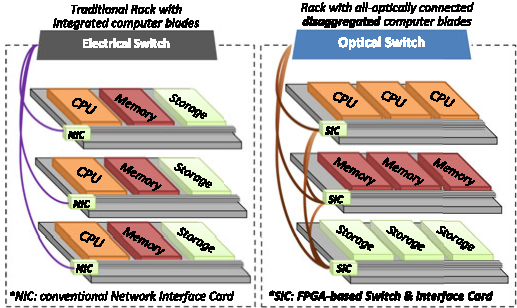
\includegraphics[width=.7\linewidth]{FPGA-sic.pdf}
  \caption{Disaggregated blades optical communication}
  \label{fig:sic}
\end{figure}

 
%%% Local Variables:
%%% mode: latex
%%% TeX-master: "main"
%%% End:
